Generally, we seek the ambisonics signals, $a_n$, up to order $L_\text{out}$, that describe the sound field in the vicinity of the listener, located at $\vec{r}_0$.
Using \eqnref{eq:02_Acoustical_Theory:Finite_Order_Expansion}, this potential field is given by
\begin{equation}\label{eq:03_Navigation_Techniques:Output_Potential_Field}
\psi(k,\vec{r} + \vec{r}_0) = \sum_{n=0}^{N_\text{out} - 1} 4\pi (-i)^l A_n(k) j_l(kr) \frac{Y_n(\hat{r})}{\|Y_n\|^2} ,
\end{equation}
where $N_\text{out} = (L_\text{out} + 1)^2$ and $A_n = \mathcal{F} \left[ a_n \right]$.

We take as inputs to each navigational method a set of measured (or synthesized) ambisonics signals, $b_n$, up to order $L_\text{in}$, that describe the sound field in the vicinity of the microphone (either real or virtual), which is located at $\vec{u}$.
Again using \eqnref{eq:02_Acoustical_Theory:Finite_Order_Expansion}, this potential field is given by
\begin{equation}\label{eq:03_Navigation_Techniques:Input_Potential_Field}
\psi(k,\vec{r} + \vec{u}) = \sum_{n=0}^{N_\text{in} - 1} 4\pi (-i)^l B_n(k) j_l(kr) \frac{Y_n(\hat{r})}{\|Y_n\|^2} ,
\end{equation}
where $N_\text{in} = (L_\text{in} + 1)^2$ and $B_n = \mathcal{F} \left[ b_n \right]$.
Thus, estimation of $a_n$ from $b_n$ amounts to a translation from the position of the microphone, $\vec{u}$, along the vector $\vec{r}_0 - \vec{u}$, as illustrated in \figref{fig:03_Navigation_Techniques:Problem_Formulation}.

% Diagram of source/mic positions
\begin{figure}[t]
\centering
  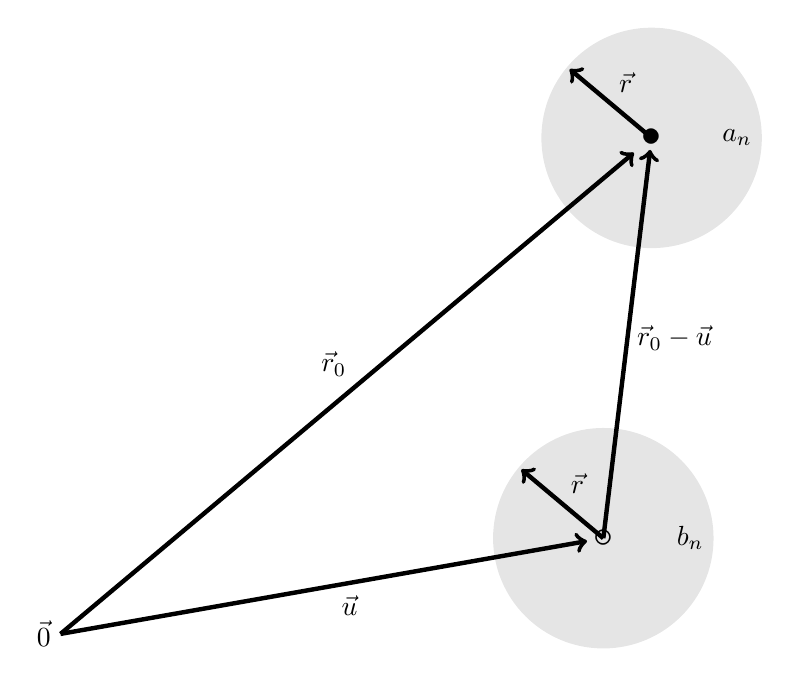
\begin{tikzpicture}[scale=5]
% Parameters
\def\lengthscale{1.4};
\def\radius{0.2*\lengthscale}
\def\arrowStart{0};
\def\arrowScale{0.97};

\pgfmathsetmacro\evalX{cos(140)*\radius}
\pgfmathsetmacro\evalY{sin(140)*\radius}

\pgfmathsetmacro\micX{cos(10)*\lengthscale}
\pgfmathsetmacro\micY{sin(10)*\lengthscale}

\pgfmathsetmacro\listenerX{cos(40)*1.4*\lengthscale}
\pgfmathsetmacro\listenerY{sin(40)*1.4*\lengthscale}

% Arrows
%\draw[ultra thick,->] ({\arrowStart*\evalX},{\arrowStart*\evalY}) -- (\arrowScale*\evalX,\arrowScale*\evalY);
%\node[above right] at (0.5*\evalX,0.5*\evalY){$\vec{r}$};
%\fill [color=black,opacity=0.1] (0,0) circle (\radius);

\draw[ultra thick,->] ({\arrowStart*\evalX+\micX},{\arrowStart*\evalY+\micY}) -- (\arrowScale*\evalX+\micX,\arrowScale*\evalY+\micY);
\node[above right] at (0.5*\evalX+\micX,0.5*\evalY+\micY){$\vec{r}$};
\fill [color=black,opacity=0.1] (\micX,\micY) circle (\radius);

\draw[ultra thick,->] ({\arrowStart*\evalX+\listenerX},{\arrowStart*\evalY+\listenerY}) -- (\arrowScale*\evalX+\listenerX,\arrowScale*\evalY+\listenerY);
\node[above right] at (0.5*\evalX+\listenerX,0.5*\evalY+\listenerY){$\vec{r}$};
\fill [color=black,opacity=0.1] (\listenerX,\listenerY) circle (\radius);

\draw[ultra thick,->] ({\arrowStart*\micX},{\arrowStart*\micY}) -- (\arrowScale*\micX,\arrowScale*\micY);
\node[below right] at (0.5*\micX,0.5*\micY){$\vec{u}$};

\draw[ultra thick,->] ({\arrowStart*\listenerX},{\arrowStart*\listenerY}) -- (\arrowScale*\listenerX,\arrowScale*\listenerY);
\node[above left] at (0.5*\listenerX,0.5*\listenerY){$\vec{r}_0$};

\draw[ultra thick,->] ({(\listenerX-\micX)*\arrowStart+\micX},{(\listenerY-\micY)*\arrowStart+\micY}) -- ({(\listenerX-\micX)*\arrowScale+\micX},{(\listenerY-\micY)*\arrowScale+\micY});
\node[right] at ({(\listenerX-\micX)*0.5+\micX},{(\listenerY-\micY)*0.5+\micY}){$\vec{r}_0 - \vec{u}$};

% Origin
\node[left] at (0,0){$\vec{0}$};

% Mic position
\node at (\micX,\micY){\Large $\circ$};
\node[left] at (\micX+\radius,\micY){$b_n$};

% Listener position
\node at (\listenerX,\listenerY){\Large $\bullet$};
\node[left] at (\listenerX+\radius,\listenerY){$a_n$};
\end{tikzpicture}
  \caption[Diagram of microphone and listener positions.]{
  Diagram of microphone and listener positions.
  The empty circle indicates the microphone position,
  the filled circle indicates the listener position, and
  the shaded disks indicate the regions of the sound field represented by the corresponding ambisonics expansions.}
  \label{fig:03_Navigation_Techniques:Problem_Formulation}
\end{figure}

In general, we will consider arrays of $P$ ambisonics microphones, where the $p^\text{th}$ microphone is located at $\vec{u}_p$ for $p \in [1,P]$.
For microphones of order $L_\text{in}$,\footnote{The order of the ambisonics microphone is generally determined by the number of capsules in the assembly.} each microphone captures $N_\text{in} = (L_\text{in} + 1)^2$ ambisonics signals, which we represent with a vector, $\mathbf{b}_p$.
(See \chapref{chap:02_Acoustical_Theory} for a review of ambisonics conventions and theory.)
%In general, ambisonics navigation techniques aim to approximate, up to order $L_\text{out}$ and with $N_\text{out} = (L_\text{out} + 1)^2$ terms, the exact ambisonics signals, $\mathbf{a}$, of the sound field at a listening position $\vec{r}_0$.
In the case of extrapolation methods, for which $P = 1$, we omit the subscripts for $\vec{u}_1$ and $\mathbf{b}_1$ (and instead simply use $\vec{u}$ and $\mathbf{b}$, respectively).

% include operator notation, tikz block diagram